\usepackage{ulem}


% This file is a solution template for:

% - Talk at a conference/colloquium.
% - Talk length is about 20min.
% - Style is ornate.



% Copyright 2004 by Till Tantau <tantau@users.sourceforge.net>.
%
% In principle, this file can be redistributed and/or modified under
% the terms of the GNU Public License, version 2.
%
% However, this file is supposed to be a template to be modified
% for your own needs. For this reason, if you use this file as a
% template and not specifically distribute it as part of a another
% package/program, I grant the extra permission to freely copy and
% modify this file as you see fit and even to delete this copyright
% notice. 


\mode<presentation>
{
  %\usetheme{boxes}
  %\usecolortheme{seagull}
  % or ...

  \setbeamercovered{transparent}
  % or whatever (possibly just delete it)

    \usecolortheme[named=OliveGreen]{structure} 
    \usetheme[height=7mm]{Rochester} 
    \setbeamertemplate{items}[ball] 
    \setbeamertemplate{blocks}[rounded][shadow=true]
}


\usepackage[czech]{babel}
% or whatever

\usepackage[utf8]{inputenc}
% or whatever

\usepackage{hyperref}
%\definecolor{links}{HTML}{2A1B81}
\hypersetup{colorlinks,linkcolor=OliveGreen,urlcolor=OliveGreen}

\usepackage{times}
% \usepackage[T1]{fontenc}
% Or whatever. Note that the encoding and the font should match. If T1
% does not look nice, try deleting the line with the fontenc.



% If you have a file called "university-logo-filename.xxx", where xxx
% is a graphic format that can be processed by latex or pdflatex,
% resp., then you can add a logo as follows:

%\pgfdeclareimage[height=1.cm]{conference-logo}{images/220px-Wikimedia_Czech_Republic-logo.svg.png}
%\pgfdeclareimage[height=1.cm]{osm-logo}{images/osm_logo-79d71f6a51b0e6a724a570834c07d828.png}
%\logo{\pgfuseimage{conference-logo}}



% Delete this, if you do not want the table of contents to pop up at
% the beginning of each subsection:
\mode<presentation>
\AtBeginSection[]
{
%\logo{\pgfuseimage{conference-logo}}
  \begin{frame}<beamer>{TOC}
    \tableofcontents[currentsection,currentsubsection]
  \end{frame}
}


% If you wish to uncover everything in a step-wise fashion, uncomment
% the following command: 

%\beamerdefaultoverlayspecification{<+->}


\subtitle {Wiki-pohled na Geodata}



\begin{document}


\title[OpenStreetMap] % (optional, use only with long paper titles)
{OpenStreetMap}

\mode*

\author[J. Čepický] % (optional, use only with lots of authors)
{Jáchym~Čepický\inst{1}}
% - Give the names in the same order as the appear in the paper.
% - Use the \inst{?} command only if the authors have different
%   affiliation.

\institute % (optional, but mostly needed)
{
  \inst{1}%
  Geosense s.r.o.
  \url{http://geosense.cz}\\
}
  
% - Use the \inst command only if there are several affiliations.
% - Keep it simple, no one is interested in your street address.

\date[] % (optional, should be abbreviation of conference name)
{Wikikonference 2013, Praha}
% - Either use conference name or its abbreviation.
% - Not really informative to the audience, more for people (including
%   yourself) who are reading the slides online

\maketitle
\institutename
Geosense s.r.o, Kudrnatka 17, 182 82 Praha 8

\begin{abstract}

\noindent ASDF ASADSF AS ASS

\end{abstract}

\begin{frame}
  \titlepage
\end{frame}

\begin{frame}{TOC}
  \tableofcontents
  % You might wish to add the option [pausesections]
\end{frame}


% Structuring a talk is a difficult task and the following structure
% may not be suitable. Here are some rules that apply for this
% solution: 

% - Exactly two or three sections (other than the summary).
% - At *most* three subsections per section.
% - Talk about 30s to 2min per frame. So there should be between about
%   15 and 30 frames, all told.

% - A conference audience is likely to know very little of what you
%   are going to talk about. So *simplify*!
% - In a 20min talk, getting the main ideas across is hard
%   enough. Leave out details, even if it means being less precise than
%   you think necessary.
% - If you omit details that are vital to the proof/implementation,
%   just say so once. Everybody will be happy with that.


%\begin{frame}{Jáchym Čepický}
%  % - A title should summarize the slide in an understandable fashion
%  %   for anyone how does not follow everything on the slide itself.
%  Jáchym Čepický
%
%  \begin{columns}
%  \column{0.7\textwidth}
%    \begin{itemize} 
%        \item Lesník
%        \item OpenSource GIS vývojář a uživatel - GRASS, OpenLayers, PyWPS, \dots
%        \item Člen představenstva Open Source Geospatial Foundation (\href{http://osgeo.org}{OSGeo.org})
%        \item \href{http://bnhelp.cz}{Help Service - Remote Sensing}
%              \href{http://ccss.cz}{Czech Center for Science and Society}
%              \href{http://geosense.cz}{Geosense}
%        \item \href{http://twitter.com/jachymc}{@jachymc}
%            \href{http://les-ejk.cz}{http://les-ejk.cz}
%            \href{http://www.openstreetmap.org/user/jachymc}{http://www.openstreetmap.org/user/jachymc}
%    \end{itemize}
%    \column{0.3\textwidth}
%    
\includegraphics[width=0.75\textwidth]{images/profil2.jpg}
%    \end{columns}
%\end{frame}
%
%\begin{frame}{Jáchym Čepický}
%    \begin{block}{}
%        Ani jeden článek na cs.wikipedia.org
%    \end{block}
%\end{frame}
%
%\logo{\pgfuseimage{osm-logo}}
%\section{Co je OpenStreetMap}
%
%\begin{frame}{OpenStreetMap}
%    \begin{block}{OpenStreetMap}
%    je projekt zaměřený na vytváření svobodných geografických dat. U většiny
%    ostatních volně dostupných map je ale užívání technicky a právně omezeno.
%    Proto vznikl tento projekt, aby umožnil lidem volně nakládat s geografickými
%    daty, používat je neobvyklými způsoby a v neposlední řadě, aby byla data
%    dostupná v aktualizované a platné podobě bez dalších nákladů a omezení.
%    \end{block}
%    \href{https://en.wikipedia.org/wiki/OpenStreetMap}{https://en.wikipedia.org/wiki/OpenStreetMap}\\
%    \href{https://cs.wikipedia.org/wiki/Openstreetmap}{https://cs.wikipedia.org/wiki/Openstreetmap}
%\end{frame}
%
%\begin{frame}{OpenStreetMap}
%    \begin{center}
%        {\em WIKIZACE} Geodat
%        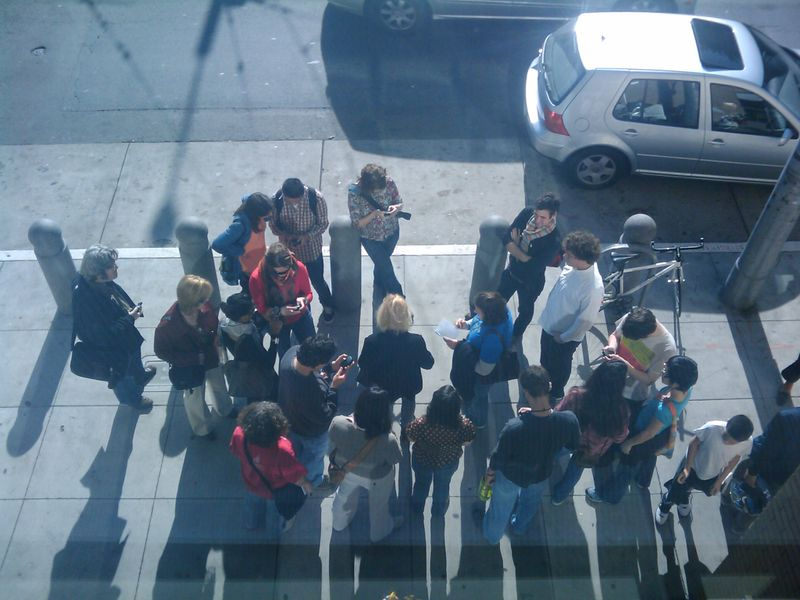
\includegraphics[width=\textheight]{images/mapping.jpg}
%    \end{center}
%\end{frame}
%
%\begin{frame}{Historie}
%       \begin{itemize}
%            \item 2004 - Steven Coast zaregistroval doménu
%            \item 2005 - MediaWiki, 1000 uživatelů
%            \item 2006 - JOSM 1.0, Map Features, OSM Foundation, Mapnik, povolení používat Yahoo! satelitní mapy
%            \item 2007 - První State of the Map, 5mil silnic a cest, 10~000 uživatelů, improty z velkých datasetů (AND, Tiger)
%            \item 2010 - Povolení používat Bing letecké snímky
%            \item 2012 - Změna lince na ODdl
%            \item 2013 - 1~000~000 registrovaných uživatelů
%       \end{itemize}
%\end{frame}
%
%\begin{frame}{OpenStreetMap}
%WIKIZACE Geodat?
%    \uncover<1>{
%        \begin{itemize}
%            \item \emph{Sbírejte data}, nahrajte data z vaší GPS
%            \item \emph{Editujte} mapu, přidávejte atributy k existujícím objektům
%            \item \emph{Sledujte změny} na mapě
%        \end{itemize}
%}
%\end{frame}
%
%\begin{frame}{Wikizace Geodat}
%    Sbírejte data
%    \begin{center}
%        \only<1>{ 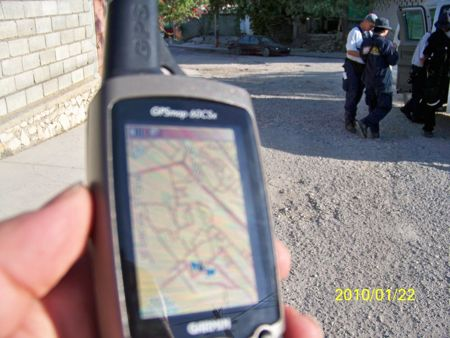
\includegraphics[width=\textheight]{images/OpenStreetMap_on_a_Garmin_in_Haiti.jpg} }
%        \only<2>{ 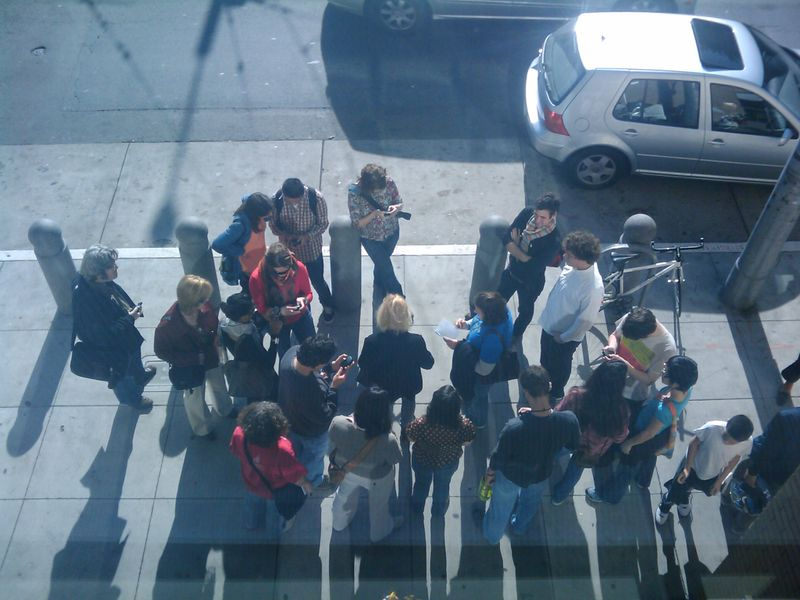
\includegraphics[width=\textheight]{images/800px-Mappers-learning-to-gps.jpg} }
%        \only<3>{ 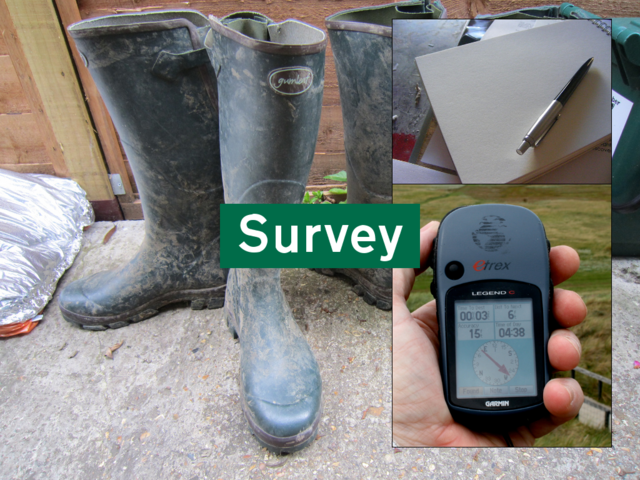
\includegraphics[width=\textheight]{images/osm-06-survey.png} }
%        \only<4>{ 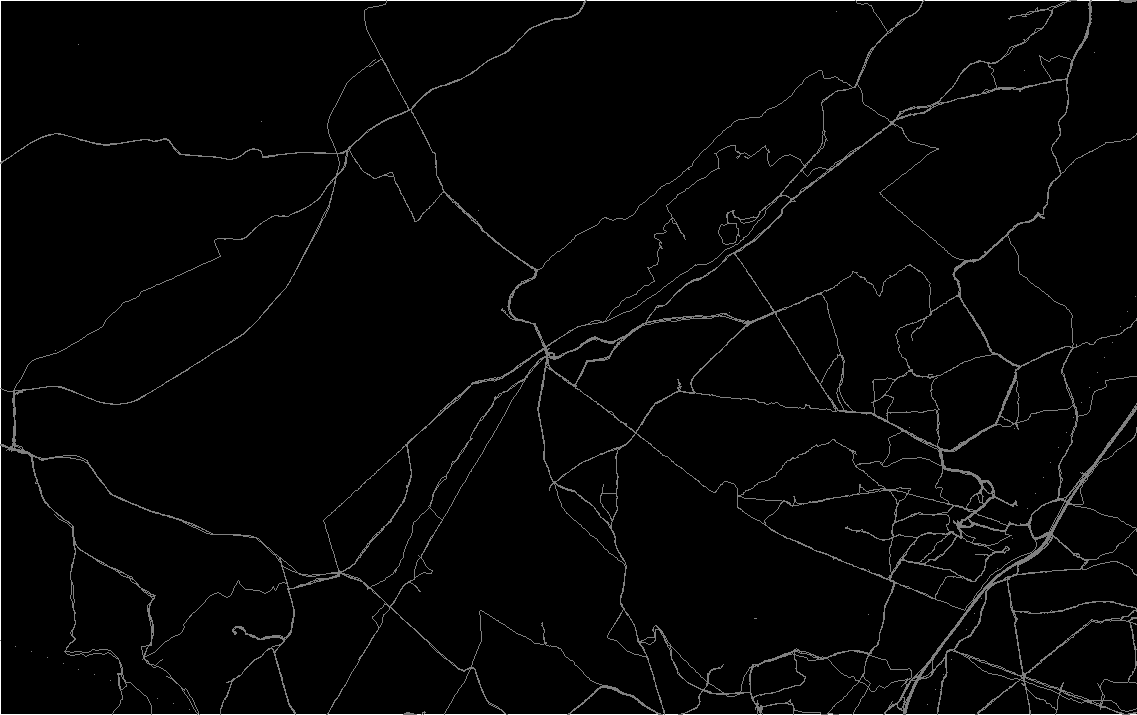
\includegraphics[width=\textheight]{images/tracs.png} }
%        \only<5>{ 
\includegraphics[width=\textheight]{images/picture-0.png} }
%    \end{center}
%\end{frame}
%
%\begin{frame}{Wikizace Geodat}
%    Sledujte změny
%    \only<1>{
%    \begin{center}
%        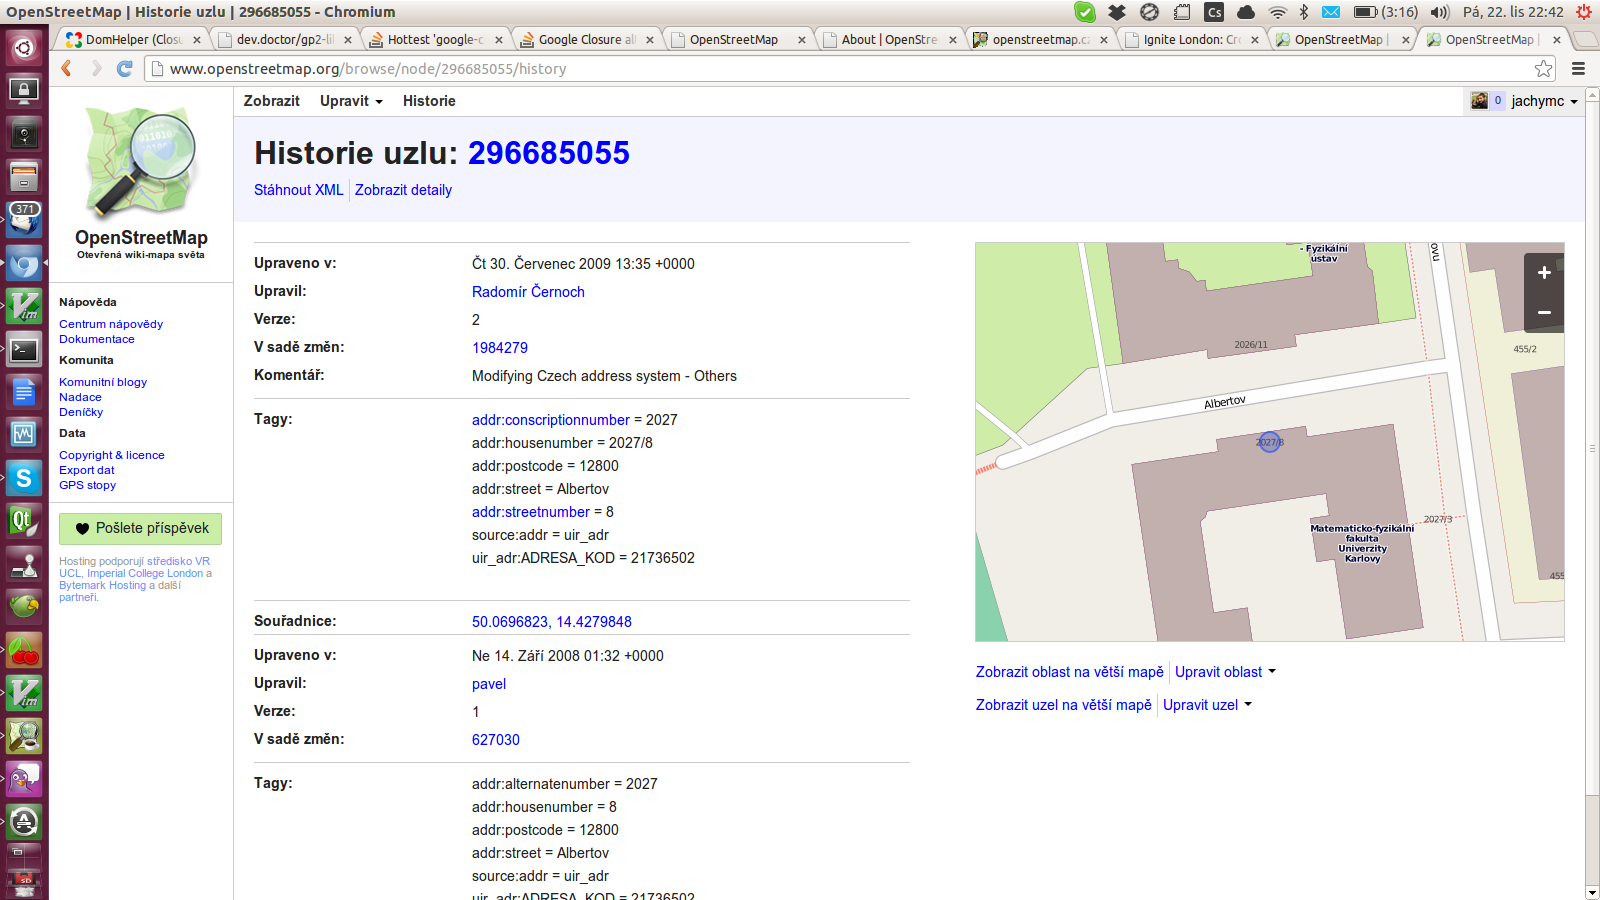
\includegraphics[width=\textheight]{images/point-history.png}
%    \end{center}
%}
%\only<2>{
%    \begin{center}
%        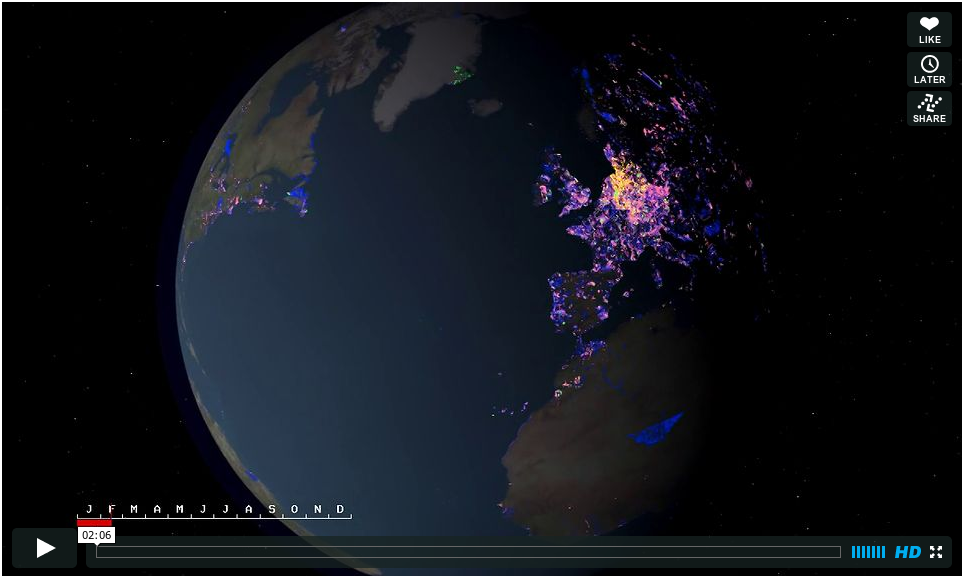
\includegraphics[width=\textheight]{images/year-of-mapping.png}\\
%        \href{http://vimeo.com/56374742}{2012 Year of edits} (video)
%    \end{center}
%}
%\end{frame}
%
%\begin{frame}{Wikizace Geodat}
%    Používejte data
%    \begin{center}
%        \only<1>{
%            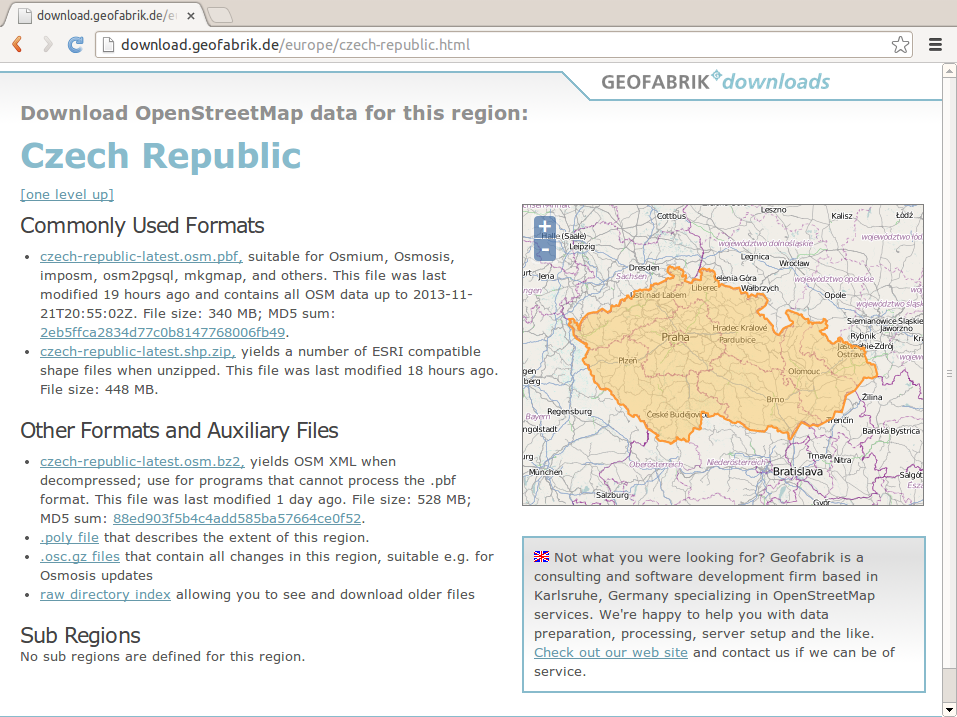
\includegraphics[width=\textwidth]{images/geofabrik.png}\\
%            \href{http://download.geofabrik.de}{download.geofabrik.de}\\
%            ČR: 340 MB, SK: 125 MB
%        }
%        \only<2>{
%        \begin{flushleft}
%             \$ osm2pgsql file.osm
%        \end{flushleft}
%        }
%        \only<3>{
%            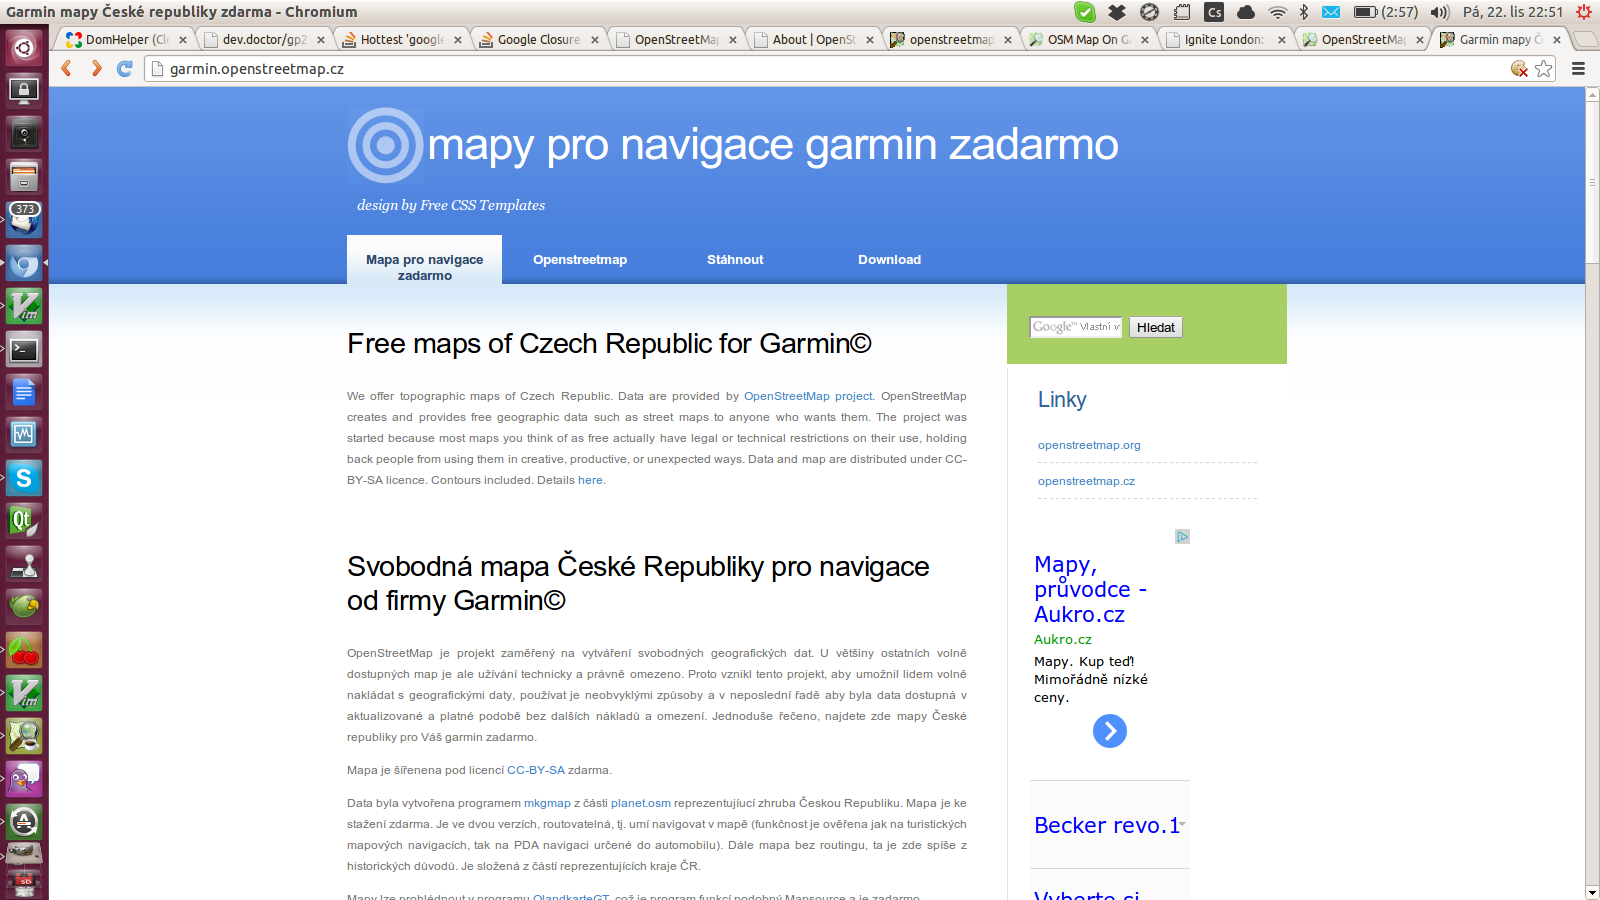
\includegraphics[width=\textwidth]{images/garmin.png}\\
%            \href{http://garmin.openstreetmap.cz/}{http://garmin.openstreetmap.cz/}
%        }
%        \only<4>{
%            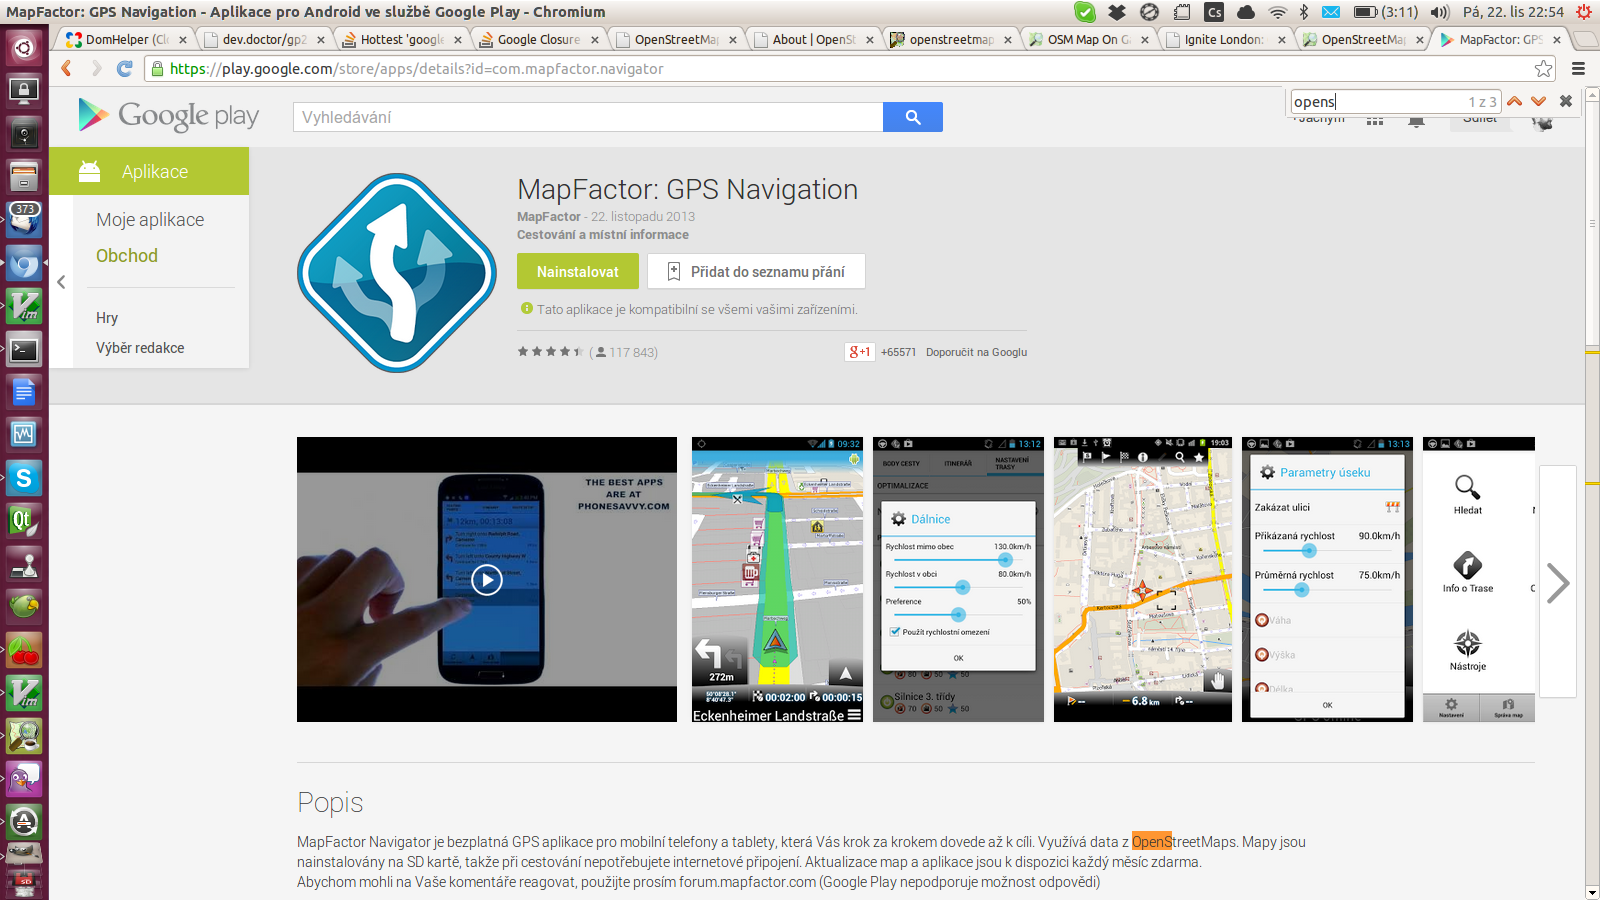
\includegraphics[width=\textwidth]{images/android.png}\\
%            \href{http://wiki.openstreetmap.org/wiki/Android}{http://wiki.openstreetmap.org/wiki/Android}
%        }
%        \only<5>{
%            
\includegraphics[width=\textwidth]{images/mapbox.png}\\
%            \href{http://mapbox.com}{http://mapbox.com}
%        }
%        \only<6>{
%            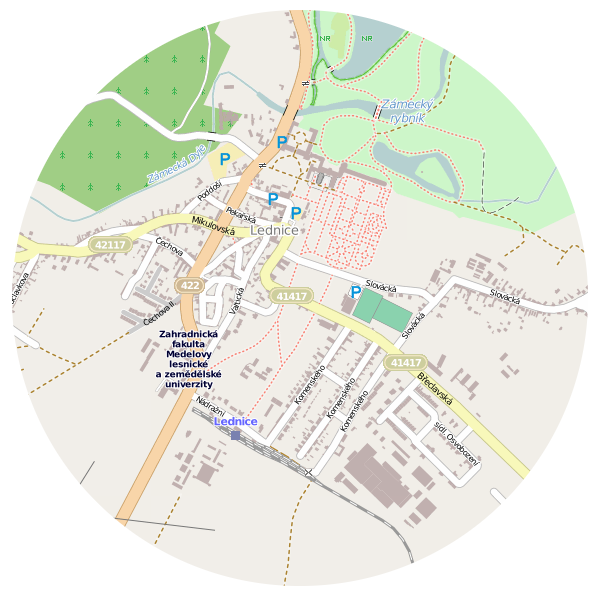
\includegraphics[width=\textwidth]{images/osm.png}\\
%            \href{http://openstreetmap.org}{http://openstreetmap.org}
%        }
%        \only<7>{
%            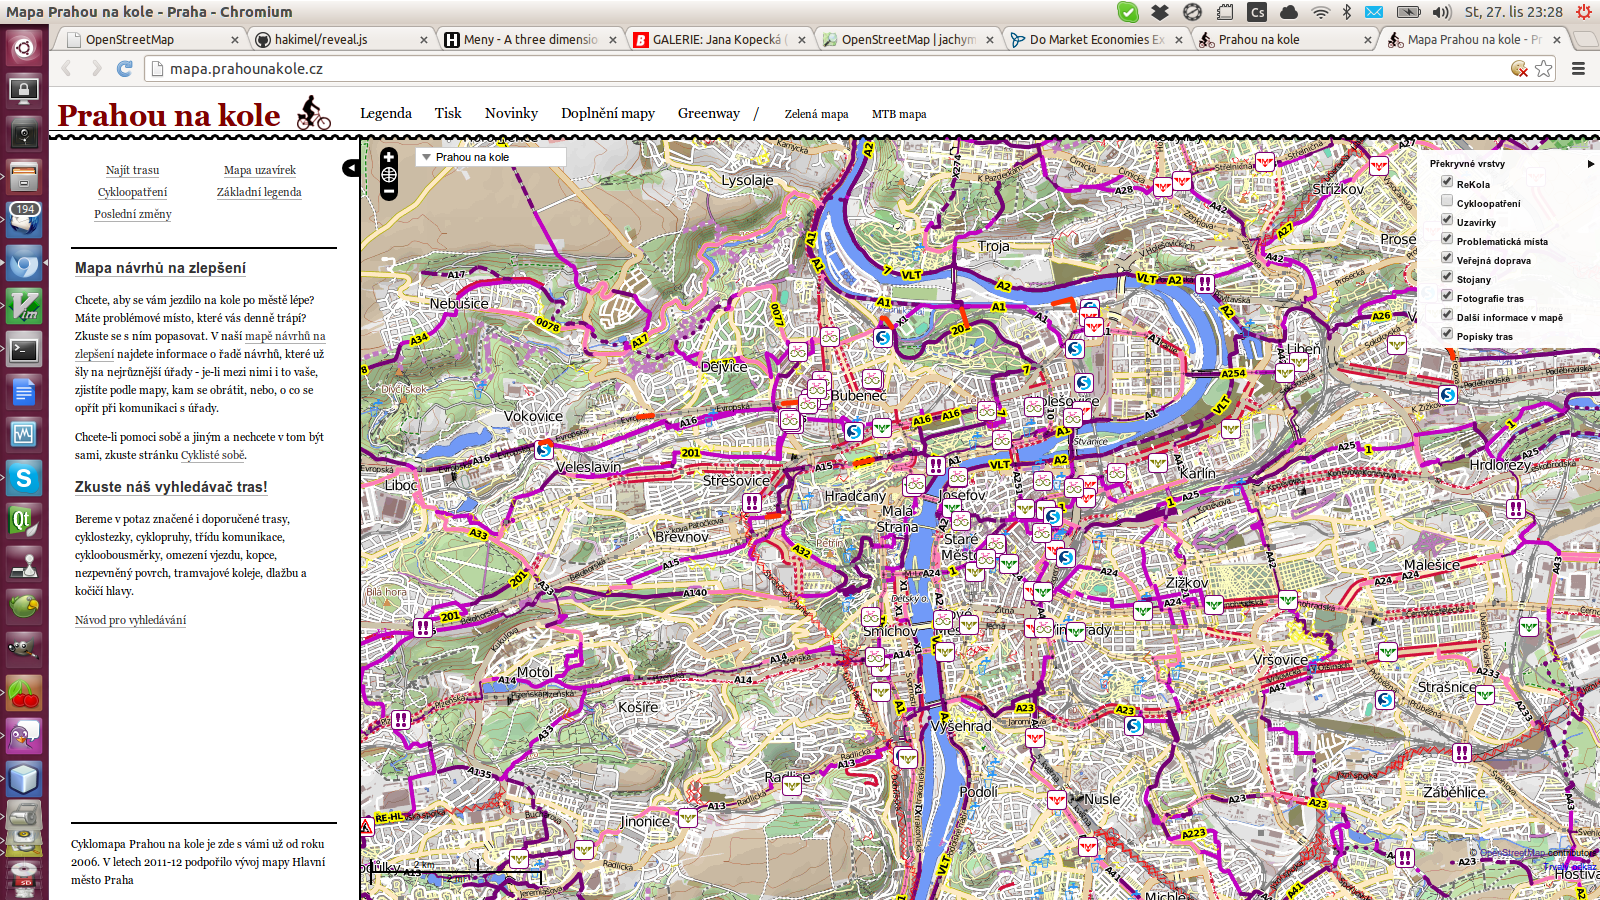
\includegraphics[width=\textwidth]{images/prahou.png}\\
%            \href{http://prahounakole.cz}{http://prahounakole.cz}
%        }
%    \end{center}
%\end{frame}
%
%\section{To je všechno?}
%\begin{frame}
%\only<1>{
%    \begin{itemize}
%        \item Co se s tím dá ještě dělat?
%        \item Co můžu dělat pro OSM, aby bylo lepší?
%    \end{itemize}
%}
%\only<2>{
%        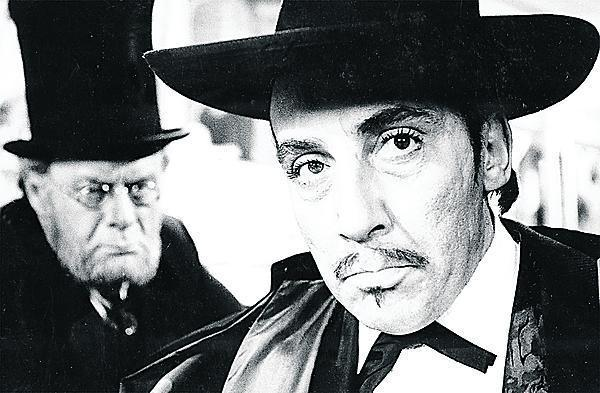
\includegraphics[width=\textwidth]{images/padouch.jpg}\\
%        Padouch nebo hrdina, my jsme jedna rodina!\\
%        Náš podnik potřebuje talenty všeho druhu.
%}
%\end{frame}
%
%\begin{frame}
%Je toho víc!
%\begin{itemize}
%    \item Data mining
%    \item Coding
%    \item Donate
%\end{itemize}
%\end{frame}
%
%\begin{frame}{Data mining}
%\only<1>{
%\begin{center}
%    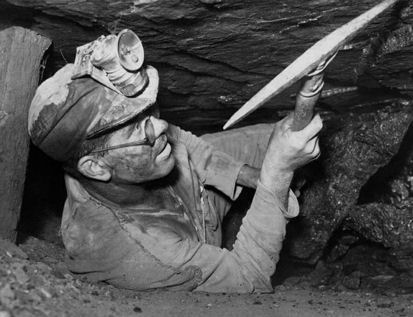
\includegraphics[width=\textwidth]{images/minig.jpg}\\
%    \href{http://www.miningartifacts.org/Kansas-Mines.html}{http://www.miningartifacts.org/Kansas-Mines.html}
%\end{center}
%}
%\only<2>{
%    \begin{itemize}
%           \item Katastrální mapy
%           \item Importy z veřejných datových zdrojů
%           \item RUIAN (registr územní identifikace, adres a nemovitostí)
%           \item Automatické získávání dat z webových služeb
%           \item \dots
%    \end{itemize}
%}
%\end{frame}
%
%\begin{frame}{Coding}
%\only<1>{
%    \begin{center}
%        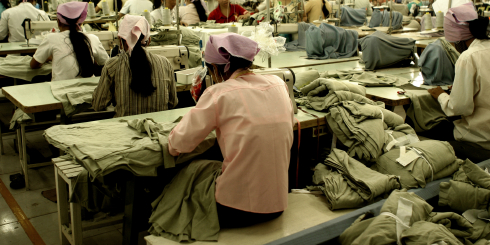
\includegraphics[width=\textwidth]{images/coding.jpg}\\
%        \href{http://blog.tifwe.org/do-market-economies-exploit-or-liberate/}{http://blog.tifwe.org/do-market-economies-exploit-or-liberate/}
%    \end{center}
%}
%\only<2>{
%
%    \begin{itemize}
%        \item Práce na editorech (JOSM), jejich zásuvných modulech
%        \item Automatické importní skripty
%        \item Automatické opravy
%        \item Vývoj jádra OSM
%    \end{itemize}
%}
%\end{frame}
%
%\begin{frame}{Donation}
%\only<1>{
%    \begin{center}
%        
\includegraphics[width=\textwidth]{images/donate.jpg}\\
%    \end{center}
%}
%\only<2>{
%    \begin{itemize}
%        \item Help Service - Remote Sensing: import silnic 1 a 2 tříd
%        \item Ústav pro hospodářskou úpravu lesů: WMS Lesů, zpřístupnění leteckých snímků, \dots 
%        \item Microsoft Bing! Maps, Yahoo Maps, \dots
%    \end{itemize}
%}
%\end{frame}
%
%\section{Organizace}
%\begin{frame}{OSM Foundation}
%    \begin{itemize}
%        \item Nezisková organizace registrovaná ve Spojeném království
%        \item Má na starosti servery
%        \item Fund-raising
%        \item Výroční konference State of the map
%    \end{itemize}
%\end{frame}
%
%\begin{frame}{Licence}
%    \begin{itemize}
%        \item Použití dat je zdarma
%        \item Musí se zobrazit upozornění, že data jsou z OSM
%        \item Veřejně dostupná odvozená díla nechť jsou zpřístupněna pomocí stejné licence
%    \end{itemize}
%    \emph{Share-alike}
%\end{frame}
%
%\begin{frame}{User groups}
%    \#cooperation, \#social, \#fun
%\end{frame}
%
%\begin{frame}{HOT}
%\begin{block}{Humanitarian OpenStreetMap Team}
%[H.O.T.] is a new initiative to apply the principles
%of open source and open data sharing towards humanitarian response and economic
%development.
%\end{block}
%\end{frame}
%
%\begin{frame}{HOT}
%\begin{center}
%        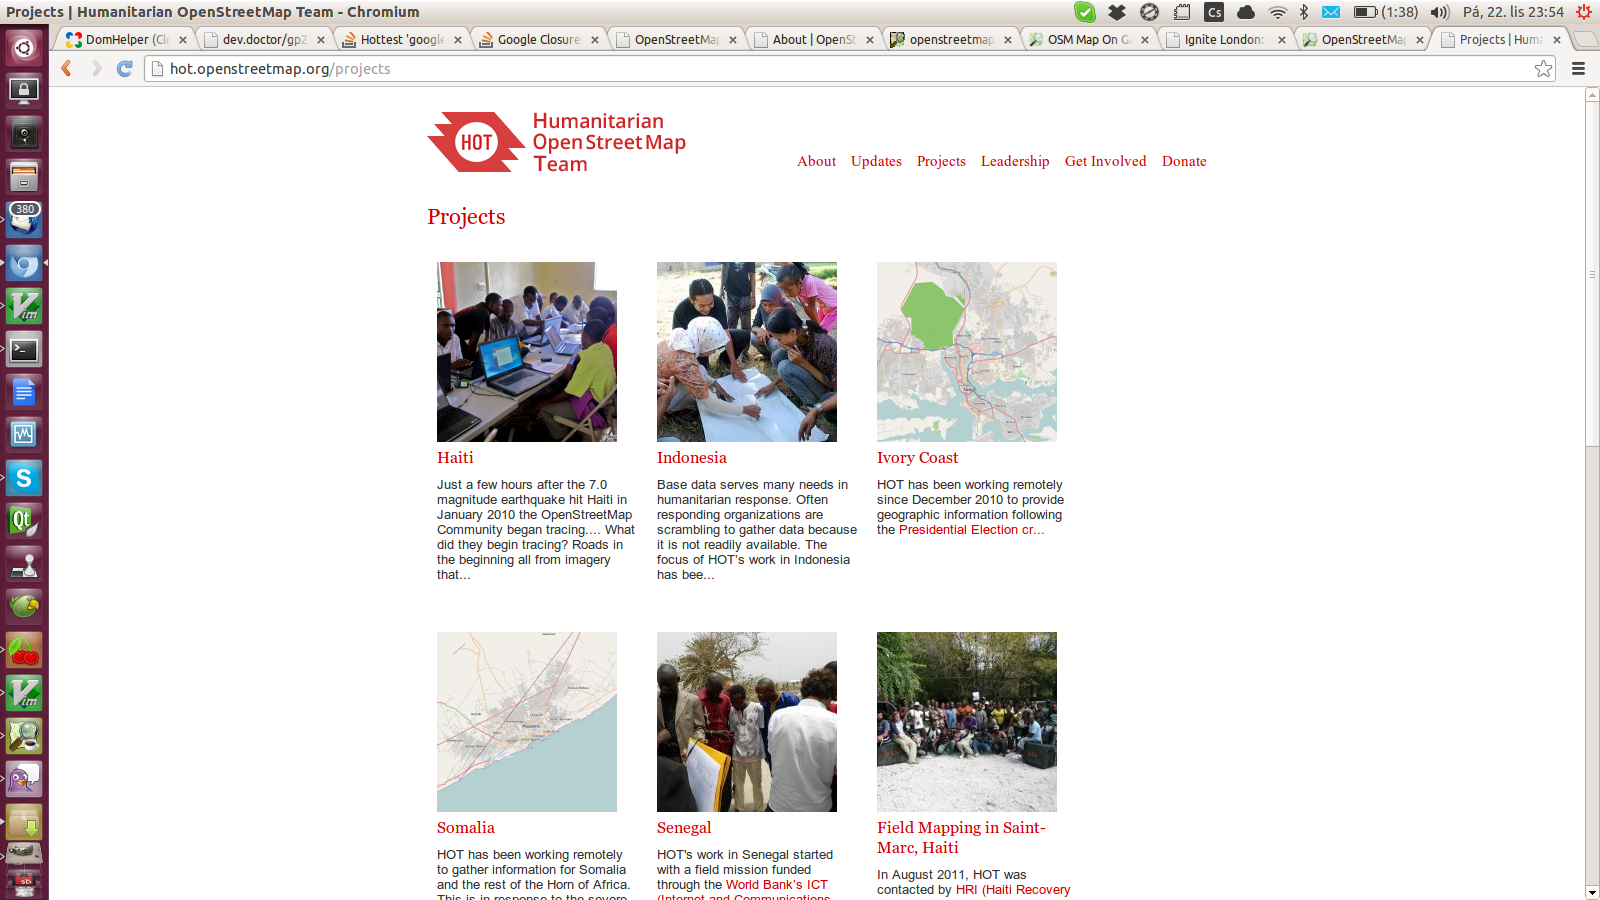
\includegraphics[width=\textwidth]{images/hot.png}\\
%        \href{http://vimeo.com/9182869}{OpenStreetMap - Project Haiti} (video)
%\end{center}
%\end{frame}
%
%\section{Česká republika}
%\begin{frame}
%    \begin{itemize}
%        \item Aktivní komunita
%        \item Exporty pro GPS Garmin
%        \item Locus
%        \item UHUL, KČT, OpenData movement, ...
%    \end{itemize}
%\end{frame}
%
%\section{Wikipedia vs. OSM}
%\begin{frame}Wikipedia vs. OSM}
%    \
%\end{frame}

\section*{Závěr}
\begin{frame}
    Happy mapping!\\
    ~
    \\
    jachym.cepicky@gmail.com\\
    http://les-ejk.cz\\
    @jachymc
\end{frame}

\end{document}
